\documentclass[twocolumn]{article}
\usepackage{graphicx}
\usepackage{amsmath}
\usepackage{hyperref}
\usepackage{xspace}

\usepackage[natbib=true,backend=biber,uniquename=init,giveninits=true]{biblatex}

\addbibresource{bibl.bib}
\newcommand\erf{\ensuremath{\mathrm{erf}}\xspace}
\newcommand\erfi{\ensuremath{\mathrm{erfi}}\xspace}
\newcommand\erfc{\ensuremath{\mathrm{erfc}}\xspace}

\newcommand\dx[1]{\,\text{d}#1}

\author{Mark L. Winther}
\title{The Bessel function}

\begin{document}
\maketitle


\begin{figure}[ht]
	\centering
	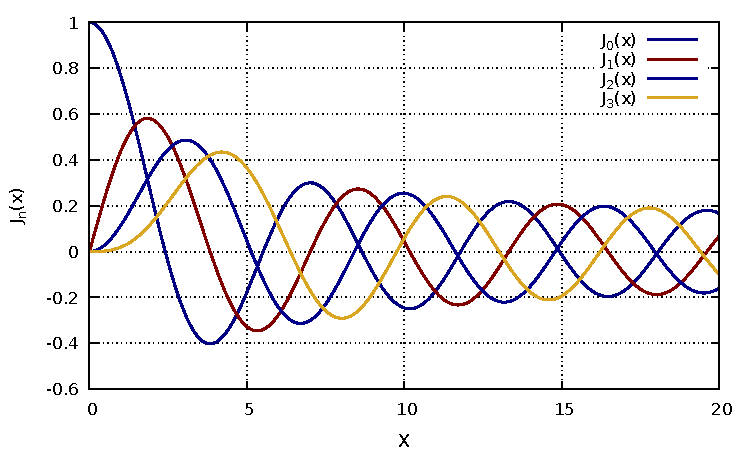
\includegraphics[width=\linewidth]{fig.pdf}
	\caption{The numerically solved Bessel function, for a range of x and n.}
	\label{fig:1}
\end{figure}

\begin{figure}[ht]
	\centering
	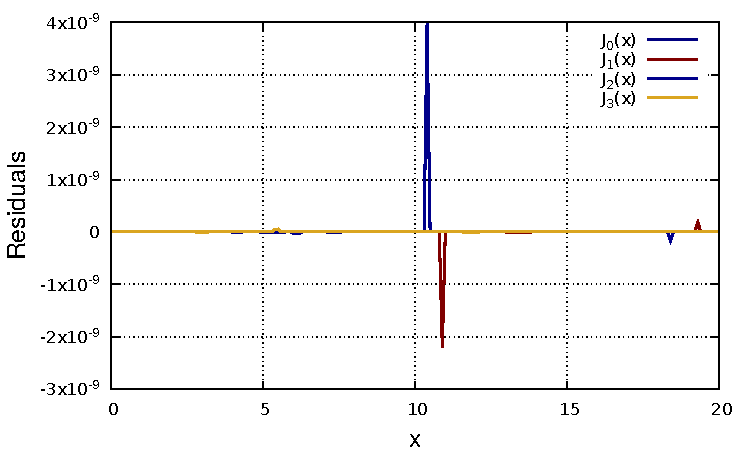
\includegraphics[width=\linewidth]{fig2.pdf}
	\caption{The residuals of the numerically solved Bessel function, for a range of x and n.}
	\label{fig:2}
\end{figure}

\cite{wiki}


\printbibliography

\end{document}
